This chapter illustrates an example of applying the proposed certification scheme to real software, showing how the manufacturer could benefit from such a solution. More specifically, the next section introduces the certification target considered for the demonstration: a web service that uses open-source OpenSSL to establish secure and encrypted communications with its clients. Moreover, we show the basics of a classic approach (e.g. Common Criteria) over the new product extracting the main properties and attributes. Additionally, we focus on the OpenSSL part of the application since two major vulnerabilities affected such software in the past and are eligible for certificate invalidation, given the properties they directly affected. Finally, we show how the proposed certification scheme can be used to solve the issue and release a complementary certificate that brings the system's trustworthiness back to its original strength with the lowest effort. OpenSSL was introduced as core component of the system for two main reasons:
\begin{description}
    \item[Open-Source] It is open-source software, which allows browsing through the code (mainly written in the C language) publicly available in the official GitHub repository (https://github.com/openssl/openssl) and inspecting all the previous versions of the software with the relative update changes.
    \item[Vulnerabilities] Researchers found multiple exposed vulnerabilities of the software during the various years of deployment; in this thesis work, only two of them will be considered for the sake of the example, the first identified by the Common Vulnerability Scoring System (CVSS) as \texttt{CVE-2014-0224} and the second as \texttt{CVE-2016-7798}.
\end{description}

With standard approaches, the presence of such vulnerabilities in a core component would trigger the certificate revocation, obliging manufacturers to install the patches to the vulnerabilities and re-certificate the software with a full certification process, costing a considerable amount of money and time; instead, the proposed scheme would allow performing a faster and cheaper re-certification that involves only the affected aspects of the system.

%%%%%%%%%%%%%%%%%%%%%%%%%%%%%%
\section{First Certification}
\label{first}
This section illustrates how a simple web service could start its lifecycle with a strong certification process capable of delivering a long-lasting certificate. More specifically, the approach taken follows the main steps of the Common Criteria process, but, for simplicity, we ignore the selection and definition of a protection profile which would be required in a real CC scenario. The phases considered in this demonstration are the identification and description of the ToE and the simulation of what the certification report could include after the manual review and testing phases.

\subsection{Target of Evaluation}
The ToE considered for this demonstration is a web service based on OpenSSL, a robust, commercial-grade, full-featured open-source toolkit for the Transport Layer Security (TLS) protocol formerly known as the Secure Sockets Layer (SSL) protocol. The protocol implementation is based on a full-strength general-purpose cryptographic library, which can also be used stand-alone.
OpenSSL is descended from the SSLeay library developed by Eric A. Young and Tim J. Hudson [hudson1997ssleay]. The OpenSSL crypto library (\textit{libcrypto}) implements various cryptographic algorithms used in various Internet standards. The services provided by this library are used by the OpenSSL implementations of TLS and CMS (Content Management System, used for encryption and decryption of files with specific formats \cite{mckeever2003understanding}), and they have also been used to implement many other third-party products and protocols.
The functionality includes symmetric encryption, public key cryptography, key agreement, certificate handling, cryptographic hash functions, cryptographic pseudo-random number generators, Message Authentication Codes (MACs), Key Derivation Functions (KDFs), and various utilities. To keep the examples simple, the implementations shown in the next sections refer only to the OpenSSL component of the certification target.

\definecolor{Gray}{gray}{0.88}
\begin{table}[ht]
    \centering
    \begin{tabular}{||l||} 
     \hline
     \rowcolor{Gray}
     \textbf{Requirement} \\ [0.5ex] 
     \hline\hline
     Cryptographic Key Generation \\ 
     \hline
     Cryptographic Key Destruction \\
     \hline
     Cryptographic Operation - Encryption/Decryption \\
     \hline
     Cryptographic Operation - Hashing \\
     \hline
     Cryptographic Operation - Signing \\
     \hline
     Cryptographic Operation - Keyed-Hash Message Authentication\\
     \hline
     Random Bit Generation\\
     \hline
     Storage of Sensitive Data\\
     \hline
     SSH Protocol\\
     \hline
     TLS Protocol\\
     \hline
     Access Controls for Protecting User Data\\
     \hline
     Authentication Failure Handling\\
     \hline
     Multiple Authentication Mechanisms\\
     \hline
     X.509 Certificate Validation\\
     \hline
     X.509 Certificate Authentication\\
     \hline
     Management of security functions behavior\\
     \hline
     Specification of Management Functions\\
     \hline
     Access controls\\
     \hline
     Address Space Layout Randomization\\
     \hline
     Stack Buffer Overflow Protection\\
     \hline
    Software Restriction Policies\\
     \hline
     Boot Integrity\\
     \hline
     Trusted Update\\
     \hline
     Trusted channel communication\\
     \hline
     Trusted Path \\ [0.5ex]
     \hline
    \end{tabular}
    \caption{Security Requirements for the Proposed Example}
    \label{tab:SR}
\end{table}



\subsection{Security Requirements}
This paragraph identifies the security properties for the ToE, which are listed in Table \ref{tab:SR}; additionally, each property is associated with the relative attributes; for simplicity only the core attributes of the most important properties are listed below:

\begin{description}
    \item[Cryptographic Key Generation] The service shall generate asymmetric cryptographic keys in accordance with a specified cryptographic key generation algorithm (\(p_1\));
    \begin{itemize}
        \item RSA schemes using cryptographic key sizes of 2048-bit or greater (\(a_1\)).
    \end{itemize}
    \item[Cryptographic Key Destruction] The service shall destroy cryptographic keys and key material in accordance with a specified cryptographic key destruction method (\(p_2\));
    \begin{itemize}
        \item For volatile memory, the destruction shall be executed by a single overwrite consisting of zeroes (\(a_2\));
        \item For non-volatile memory that consists of the invocation of an interface provided by the underlying platform that logically addresses the storage location of the key and performs specified number (default of 3) of overwrites consisting of a pseudo-random pattern (\(a_3\));
    \end{itemize}
    \item[Cryptographic Operation - Encryption/Decryption] The service shall perform encryption and decryption services for data in accordance with a specified cryptographic algorithm (\(p_3\));
    \begin{itemize}
        \item AES-128-CBC (\(a_4\))
        \item AES-192-CBC (\(a_5\))
        \item AES-256-CBC (\(a_6\))
        \item AES-128-GCM (\(a_7\))
        \item AES-192-GCM (\(a_8\))
        \item AES-256-GCM (\(a_9\))
    \end{itemize}
    \item[Cryptographic Operation - Hashing] The service shall perform [cryptographic hashing services] in accordance with a specified cryptographic algorithm (\(p_4\))
    \begin{itemize}
        \item SHA-256 (\(a_{10}\))
        \item SHA-384 (\(a_{11}\))
        \item SHA-512 (\(a_{12}\))
    \end{itemize}
    and message digest sizes
    \begin{itemize}
        \item 256 bits (\(a_{13}\))
        \item 384 bits (\(a_{14}\))
        \item 512 bits (\(a_{15}\))
    \end{itemize}
    \item[Cryptographic Operation - Signing] The service shall perform [cryptographic signature services (generation and verification)] in accordance with a specified cryptographic algorithm (\(p_5\))
    \begin{itemize}
        \item RSA schemes using cryptographic key sizes of 2048-bit or greater (\(a_{16}\))
    \end{itemize}
    
    \item[Random Bit Generation] The service shall perform all deterministic random bit generation (DRBG) services using a specific algorithm (\(p_6\)).
    \item Random Bit Generation )
    \begin{itemize}
       \item CTR\_DRBG (AES) (\(a_{17}\))
   \end{itemize}
    
    \item[TLS Protocol] The service shall implement TLS 1.2 supporting the following cipher suites (\(p_7\)).
    \begin{itemize}
        \item TLS\_DHE\_RSA\_WITH\_AES\_128\_CBC\_SHA256 (\(a_{18}\))
        \item TLS\_DHE\_RSA\_WITH\_AES\_256\_CBC\_SHA256 (\(a_{19}\))
        \item TLS\_DHE\_RSA\_WITH\_AES\_128\_GCM\_SHA256 (\(a_{20}\))
        \item TLS\_DHE\_RSA\_WITH\_AES\_256\_GCM\_SHA384 (\(a_{21}\))
        \item TLS\_ECDHE\_ECDSA\_WITH\_AES\_128\_CBC\_SHA256 (\(a_{22}\))
        \item TLS\_ECDHE\_ECDSA\_WITH\_AES\_128\_GCM\_SHA256 (\(a_{23}\))
        \item TLS\_ECDHE\_ECDSA\_WITH\_AES\_256\_GCM\_SHA384 (\(a_{24}\))
        \item TLS\_ECDHE\_RSA\_WITH\_AES\_128\_CBC\_SHA256 (\(a_{25}\))
        \item TLS\_ECDHE\_RSA\_WITH\_AES\_128\_GCM\_SHA256 (\(a_{26}\))
        \item TLS\_ECDHE\_RSA\_WITH\_AES\_256\_GCM\_SHA384 (\(a_{27}\))
    \end{itemize} 
    and implementing the correct sequence of message for the connection handshake (\(a_{28}\)).
    
   \item[Cryptographic Operation - Signing] The service shall perform cryptographic signature services (generation and verification) in accordance with a specified cryptographic algorithm (\(p_8\))
    \begin{itemize}
        \item RSA schemes using cryptographic key sizes of 2048-bit or greater (\(a_{29}\))
    \end{itemize}

\end{description}


\subsection{Evaluation Procedure and Certificate Release}
\label{firstcert}
Following the standard procedure of the Common Criteria, the next step is to identify the ToE configuration to evaluate the abovementioned properties and attributes. In this case, the tested configuration consists of a machine mounting an \texttt{AMD Ryzen 5 3600 6-Core} CPU running \texttt{Linux Ubuntu version 22.04.1} through a VMWare virtual machine. Finally, the tests can be executed to establish if the system effectively holds the identified properties and attributes. The actual testing process of this certification scheme is out of the scope of this thesis, and we assume the certification process's success leads to the certificate's release, but below, we show what the resulting certificate would look like if described using the formal models defined in Chapter \ref{cap3}. We defined the certificate as a set of pairs, each representing a micro-property and the set of evidence supporting it; more specifically, each piece of evidence aims at supporting an attribute of the micro-property. The certificate resulting from the CC process would be translated into the following formalization: 

\[\{ (p_1, \{e_1\}),(p_2, \{e_2, e_3\}),(p_3, \{e_4, \dots, e_9\}),(p_4, \{e_{10}, \dots, e_{15}\}),(p_5, \{e_{16}\}), \]
\[(p_6, \{e_{17}\}),(p_7, \{e_{18}, \dots, e_{28}\}),(p_8, \{e_{29}\}) \}\]

The resulting certificate above can ultimately be interpreted by the trigger component of the proposed certification scheme and used to compare every change the system undergoes, eventually triggering the re-certification process. Such an event has a high chance of happening when dealing with highly dynamic systems similar to the one considered in this example; in the next section, we show how a situation involving a needed re-certification could be handled using the proposed Ephemeral Certification.




\section{Ephemeral Certification}
This section illustrates a complete walkthrough of the proposed certification scheme over the web service introduced in the previous section. We note that the service is based on OpenSSL which underwent the OpenSSL cryptolibrary update. the following sections include all the phases described in Chapter \ref{cap3} from the analysis of the system's update, using the certificate obtained in Section \ref{firstcert}, to the release of a new certificate. Furhermore, we note that all tests were executed on the same machine configuration as in Section \ref{first} using a client-server setup that simulates how a web service would function. The diagram in figure \ref{fig:proc_prop} shows a simple illustration of the properties and attributes considered in the following paragraphs.

\begin{figure}[ht]
    \centering
    \fbox{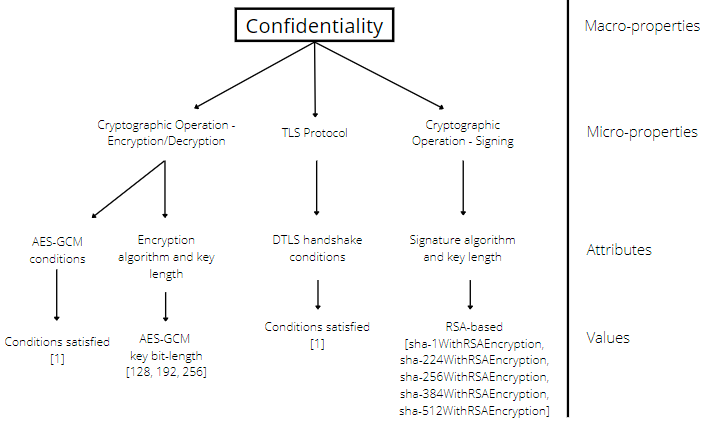
\includegraphics[scale=0.75]{images/Process_properties.png}}
    \caption{Simple illustration of the properties and attributes considered for the proposed scheme's demonstration}
    \label{fig:proc_prop}
\end{figure}



%%%%%%%%%%%%%%%%%%%%%%%%%%%%%%%%%%% 1 %%%%%%%%%%%%%%%%%%%%%%%%%%%%%%%%%%%%%%%
\subsection{Vulnerabilities Assessment and Certification Walkthrough}
\subsubsection{CVE-2014-022 - Trigger phase}
The \texttt{CVE-2014-0224} vulnerability allowed man-in-the-middle attackers \cite{conti2016survey} to use a zero-length master key in certain OpenSSL-to-OpenSSL communications and consequently hijack sessions or obtain sensitive information via a crafted TLS handshake, also known as ``CCS Injection" vulnerability \cite{CCS}; such a weakness represented a high risk for the users' privacy and the systems confidentiality macro-property.
The bug that exposed the \texttt{CVE-2014-0224} vulnerability consisted of a bad implementation of the DTLS handshake protocol \cite{DTLS}, which allowed bad actors to defeat any encryption algorithm used effortlesly; hence, the influenced property is the ability to manage cryptographic keys securely. More specifically, the server entity was allowed to accept the ChangeCipherSpec (CCS) message at timings different from the intended one; hence, the attribute of the property that will be considered is the timing of the CCS message, which must satisfy two conditions to be accepted: i) there are no fragments from the handshake uncompleted (e.g. certificate validation) and ii) the next message received is Finished; the correct sequence of the messages is shown in Figure \ref{fig:handshake}.

\begin{figure}[ht]
    \centering
    \fbox{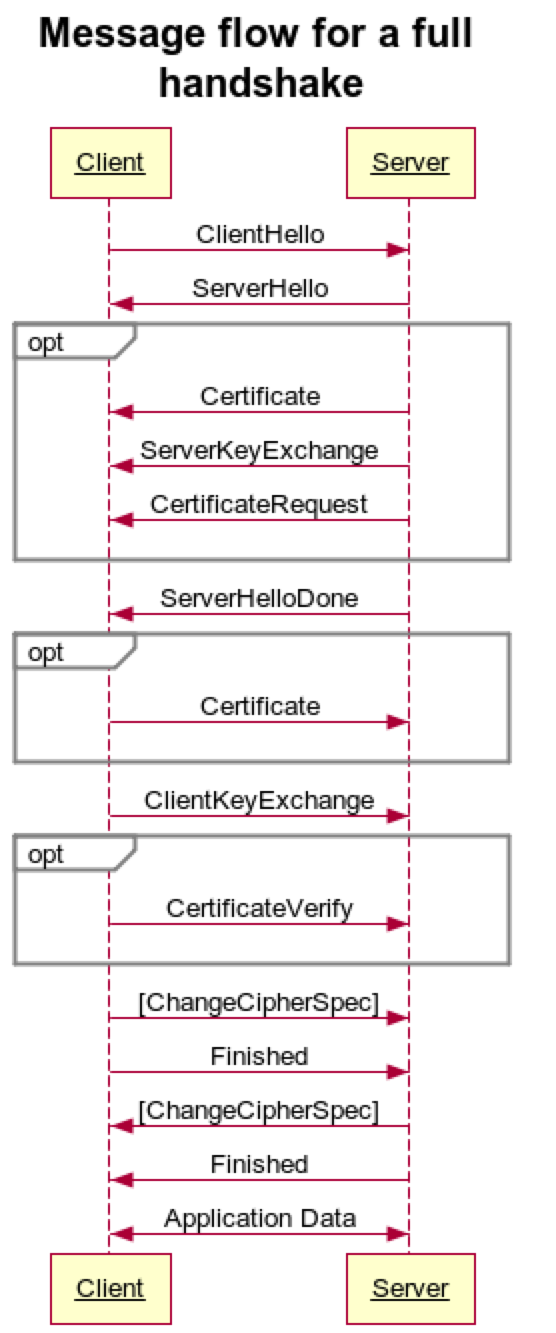
\includegraphics[scale=0.3]{images/ccs_handshake.png}}
    \caption{TLS handshake protocol messages sequence diagram}
    \label{fig:handshake}
\end{figure}


After the system receives the update, the trigger component analyses the changes, comparing the old certificates with the updated properties and attributes and extracting the following ones:
\begin{itemize}
    \item TLS Protocol (\(p_1\));
    \begin{itemize}
        \item DTLS handshake conditions (\(a_1\));
    \end{itemize}
\end{itemize}

Following the formalization of the \textit{Changes} function introduced in Section \ref{trigger}, the output of such function for this vulnerability is: \[ \{ (p_1, \{a_1\})\}\]

After listing the impacted properties and attributes and making them available, the trigger signals a manual operator that the process requires attention.

\subsubsection{CVE-2014-022 - Manual revision phase}
An expert manual operator accesses the properties and attributes through the Changes function and deals with three main tasks:
\begin{itemize}
    \item According to technological standards, the operator assigns a list of values to each attribute; in this example, they result formalized as follows:
    \begin{itemize}
        \item \(\langle a_1, [1]\rangle\);
    \end{itemize}
    
    \item According to her assumed knowledge, the operator assigns a range of scores that directly map to the values of each attribute:
    \begin{itemize}
        \item {[20]} for \(a_1\);
    \end{itemize}
\end{itemize}

%%%%%%%%%%%%%%%%%%%%%%%%%%%%%%%%%%% 2 %%%%%%%%%%%%%%%%%%%%%%%%%%%%%%%%%%%%%%

\subsubsection{CVE-2016-779 - Trigger phase}
The \texttt{CVE-2016-7798} vulnerability affected the OpenSSL Ruby gem, which used the same initialization vector for multiple encryptions in a specific configuration; this allowed attackers to decipher encrypted messages easily \cite{vector}; this weakness, as the previous one, represented a high risk for the users' privacy and the systems confidentiality macro-property.
The bug that exposed the second vulnerability (CVE-2016-7798) consisted of a bad implementation of the Ruby Openssl gem when using the AES algorithm in Galois/Counter Mode (GCM) \cite{gcm}, which allowed each initialization vector to be used multiple times; this resulted in weak encryption of data. The issue was caused by the initialization vector being set before the key when it should have been set after it. The attributes considered in this process are the encryption algorithm (AES-GCM), the satisfaction of the requirement of having a different initialization vector every time and the correlated certificate signing algorithm, which is also affected by this issue.



After the system receives the update, the trigger component analyses the changes, comparing the old certificates with the updated properties and attributes and extracting the following properties and attributes:

\begin{itemize}
    \item Cryptographic Operation - Signing (\(p_2\));
    \begin{itemize}
        \item Signature algorithm and key length. (\(a_2\))
    \end{itemize}
    \item Cryptographic Operation - Encryption/Decryption (\(p_3\));
    \begin{itemize}
        \item AES-GCM conditions (\(a_3\));
        \item AES-GCM key length (\(a_4\)).
    \end{itemize}
\end{itemize}

Following the formalization of the \textit{Changes} function introduced in Section \ref{trigger}, the output of such function for this vulnerability is: \[ \{(p_2, \{a_2\}), (p_3, \{a_3, a_4\}) \}\]

After listing the impacted properties and attributes and making them available through the \textit{Changes} function, the trigger signals a manual operator that the process requires attention.

\subsubsection{CVE-2016-779 - Manual revision phase}
An expert manual operator accesses the properties and attributes through the Changes function and deals with three main tasks:
\begin{itemize}
    \item According to technological standards, the operator has to assign to each attribute a list of values; for this vulnerability, they result formalized as follows:
    \begin{itemize}
        \item \(\langle a_2, [\texttt{sha-1WithRSAEncryption, sha-224WithRSAEncryption,}\)
        
        \(\texttt{sha-256WithRSAEncryption, sha-384WithRSAEncryption,} \)
        
        \(\texttt{sha-512WithRSAEncryption}]\rangle\)
        \item \(\langle a_3, [1] \rangle\);
        \item \(\langle a_4, [128, 192, 256] \rangle\).
    \end{itemize}
    
    \item According to her assumed knowledge, the operator assigns a range of scores that directly map to the values of each attribute:
    \begin{itemize}
        \item {[5, 10, 20, 50, 70]} for \(a_2\).
        \item {[20]} for \(a_3\);
        \item {[5, 10, 20]} for \(a_4\).
    \end{itemize}
    
\end{itemize}


\subsubsection{Macro-properties thresholds definition}
The operator needs access to all the micro-properties and attributes that will be evaluated in order to define a threshold for each macro-property; we note that all the listed micro-properties fall into the \textit{Consistency} macro-property. Then, let us suppose that the operator assigns a threshold of 80 and a weight of 1 (1 means that the final weighted sum is ignored, the weight is meant to allow additional control over the final results, which is not needed for this example) according to her assumed knowledge. At this point, the system must compute the minimum value needed by each attribute to reach the threshold with the minimum possible effort. In this case, since the threshold is 80 and the attributes are 4, each attribute needs a score of 20 and will be tested for the corresponding value; the micro-properties result formalized as follows:
\begin{itemize}
    \item \(\langle p_1, \{ (a_1, 1 ) \} \rangle\);
    \item \(\langle p_2, \{(a_2, \texttt{sha-256WithRSAEncryption})\} \rangle\);
    \item \(\langle p_3, \{(a_3, 1), (a_4, 256)\} \rangle\).
\end{itemize}

Finally, the Confidentiality macro-property \(P_1\) results formalized as follows: \[P_1 = \langle Confidentiality, \{ (p_1, 20), (p_2, 20), (p_3, 40) \}, 80 \rangle\].

In case the system results holding such requirements, then the certificate can be released.


\subsubsection{CVE-2014-022 - Testing phase}
The testing phase for \texttt{CVE-2014-0224} is composed of a single test, which, following the test formalization of Section \ref{evmodel}, results in: \(t1 = \langle p_1, (a_1, 1, c_1) \rangle\), where \(c_1\) represents the code and commands used for this test, detailed below. The server was tested with OpenSSL version 0.9.8y, known for being vulnerable to the CCS injection attack, and version 3.0.2, which implements the security patch to the vulnerability. Both server instances were initialized with the same commands: First, it is required to generate a new key and a certificate on the server that will be used to establish a secure SSL/TLS connection with the following command:
``openssl req -x509 -newkey rsa:4096 -keyout key.pem -out cert.pem -days 365 -nodes"; the command req is used to create a self-signed test certificate with the argument x509, and the other arguments are: i) \textbf{newkey rsa:4096} generates a new private RSA key of size 4096 bits, ii) \textbf{keyout} copies the generated key into a file named key.pem, iii) \textbf{out} copies the generated certificate into a file named cert.pem, iv) \textbf{days} specifies the validity duration of the certificate and v) \textbf{nodes} avoids encrypting the generated private key.
Next, the server can be started using the following command:
``\texttt{openssl s\_server -key key.pem -cert cert.pem -accept 44330 -www}"; the command \textbf{s\_server} implements a generic SSL/TLS server which accepts connections from remote clients speaking SSL/TLS, and the arguments are: i) \textbf{key} specifies the private key to use, ii) \textbf{cert} specifies the certificate file to use, iii) \textbf{accept} specifies the port to listen on for connections, and iv) \textbf{www} sets the server to send a status message back to the client when it connects.

On the client side, executing a script designed to check if the server is vulnerable to the CCS injection exploit is sufficient; such a script is publicly available on [nmap.org website] and uses the open-source tool Nmap \cite{nmap}. The script works by sending a `\textit{ChangeCipherSpec}' message out of order and checking whether the server returns a `\textit{UNEXPECTED\_MESSAGE}' alert record or not. Since a non-patched server would simply accept this message, the CCS packet is sent twice in order to force an alert from the server. The server is vulnerable if the alert type is different from `\textit{UNEXPECTED\_MESSAGE}'; the script is shown in appendix \ref{ccs}. The output provided by the script is the following for the vulnerable server test:  

\begin{verbatim}
Starting Nmap 7.80 ( https://nmap.org ) at 2022-09-17 19:23 CEST
Nmap scan report for localhost (127.0.0.1)
Host is up (0.00012s latency).

PORT      STATE SERVICE
44330/tcp open  unknown
| ssl-ccs-injection: 
|   VULNERABLE:
|   SSL/TLS MITM vulnerability (CCS Injection)
|     State: VULNERABLE
|     Risk factor: High
|      OpenSSL before 0.9.8za, 1.0.0 before 1.0.0m, and 1.0.1 before 1.0.1h
|      does not properly restrict processing of ChangeCipherSpec messages,
|      which allows man-in-the-middle attackers to trigger use of a zero
|      length master key in certain OpenSSL-to-OpenSSL communications, and
|      consequently hijack sessions or obtain sensitive information, via
|      a crafted TLS handshake, aka the ``CCS Injection" vulnerability.
|           
|     References:
|       http://www.cvedetails.com/cve/2014-0224
|       https://cve.mitre.org/cgi-bin/cvename.cgi?name=CVE-2014-0224
|_      http://www.openssl.org/news/secadv_20140605.txt

Nmap done: 1 IP address (1 host up) scanned in 1.18 seconds
\end{verbatim}

and the following for the patched server test:
\begin{verbatim}
Starting Nmap 7.80 ( https://nmap.org ) at 2022-09-17 19:26 CEST
Nmap scan report for localhost (127.0.0.1)
Host is up (0.000079s latency).

PORT      STATE SERVICE
44330/tcp open  unknown

Nmap done: 1 IP address (1 host up) scanned in 0.17 seconds
\end{verbatim}

The test results show that the server running OpenSSL version 3.0.2 is no longer vulnerable to the CCS injection attack, while, with version 0.9.8y, the script highlights the presence of the vulnerability.


\subsubsection{CVE-2016-779 - Testing phase}
The testing phase for \texttt{CVE-2016-7798} is composed of two tests, which, following the test formalization of Section \ref{evmodel}, result in: \(t_2 = \langle p_2, (a_2, \texttt{sha-256WithRSAEncryption}, c_2) \rangle\) and \(t_3 = \langle p_3, \{(a_3, 1, c_3), (a_4, 256, c_4)\}  \rangle\), where \(c_2, c_3\) and \(c_4\) represent the code used for this test, detailed below.

The test for the \texttt{sha-256WithRSAEncryption} signature algorithm (\(t_2\)) was executed using a client-server setup with the Ruby language; the scripts used are shown in the appendix \ref{sig}. This test aimed to verify the integrity of the system's (server) certificate when generated using the \texttt{sha-256WithRSAEncryption} algorithm. The test's steps are as follows: i) the client connects to the server and sends an \textit{`HELLO'} message, ii) the server accepts the connection and replies to the \textit{`HELLO'} message with its certificate, iii) the client receives the server's certificate and extracts the server's public key from it, iv) the client uses the server's public key to encrypt a document and sends the result to the server, v) the server receives the encrypted document and decrypts it with its private key, vi) the server uses its private key to sign the decrypted document and sends the result to the client and vii) the client receives the signed document and verifies the authenticity of the signature usign the server's public key; if such verification succeeds the test is passed.

The output of the test on the server-side is the following:
\begin{verbatim}
>> Server listening on port 44330

>> New client connected

>> Received client's HELLO message, certificate sent

>> Received document encrypted by the client with this server's public key
>> Decrypted text:
This is an example document

>> Document signed with this server's private key

>> Signed document sent to the client

>> The client terminated the connection
\end{verbatim}

and the output of the test on the client-side is the following:
\begin{verbatim}
>> Connected to the server at 127.0.0.1:44330

>> HELLO message sent

>> Received server's certificate:
-----BEGIN CERTIFICATE-----
MIIFuzCCA6OgAwIBAgIUMo/2YlijMS2n80NQTCOWYPAg8UAwDQYJKoZIhvcNAQEL
BQAwbTELMAkGA1UEBhMCaXQxCzAJBgNVBAgMAnZhMRIwEAYDVQQHDAlnYWxsYXJh
dGUxDjAMBgNVBAoMBXVuaW1pMQ8wDQYDVQQDDAZtYXR0ZW8xHDAaBgkqhkiG9w0B
CQEWDXRlb0BnbWFpbC5jb20wHhcNMjIwOTIwMTU1MzAxWhcNMjMwOTIwMTU1MzAx
WjBtMQswCQYDVQQGEwJpdDELMAkGA1UECAwCdmExEjAQBgNVBAcMCWdhbGxhcmF0
ZTEOMAwGA1UECgwFdW5pbWkxDzANBgNVBAMMBm1hdHRlbzEcMBoGCSqGSIb3DQEJ
ARYNdGVvQGdtYWlsLmNvbTCCAiIwDQYJKoZIhvcNAQEBBQADggIPADCCAgoCggIB
ALi7TCyfIx9vJX4aofx0KlLwBctf+oKDn+xUduDJh43d31WvBGlomfUYxGGzlsWm
UXUaJ+mNf57kEra+zoIPVF2vIExr0CD7HpaYzRnWQGb5PFQkSppmfpMOzRTu94R+
7d47rMSNKY8g0G3gwhZMcVViBKUmDmoUccn1piW4s2Ur+esWfvb9qhBHJ8uqhL7h
2sFStjZKhIiMyW0zJcepnD9QikNme76X2fmYPS6pb7oMhdYurj4ILbqJctazmLMi
w2VLas74eVD9SA9WcszNIgNUBh7adTXHHPM9t6YGzYLGkn0PQ+vi5BqKPaTWdY8x
s6OFgh37klDPgvOAKDCVMRUkGSRzOpB/0k5wu6t9R6XY4mpa3BTxvEoee3B6Wx6z
WRJuemjx26JGw7D+enDXEw8+DCj532so1m0ytHKTrQd0NI5xztUJUdFE1e0/EnOR
m0Dq9/FYE1acpJnNo+FRApD1zcd08UdSF1DNNbVv27EVWCVHJFu7BlSl6tHvFroW
pSMkZtk2JVmkkAfrqJDdMhz7EZ65w9NSYy7DQEhYiYequnVei7lAHRVONJ3nQffw
EasNyDKG37WwarMFoqib4/8GDMtU0j/osQp9UAslMEBYQHFEakQRq8It5ACsznkw
AZy7ojZiQSkFdjqJ7cDyJhdiQcv9dKc0kIORKbZQ/17rAgMBAAGjUzBRMB0GA1Ud
DgQWBBTatWBPOpLFToMvhyV4q3vcRG+cQTAfBgNVHSMEGDAWgBTatWBPOpLFToMv
hyV4q3vcRG+cQTAPBgNVHRMBAf8EBTADAQH/MA0GCSqGSIb3DQEBCwUAA4ICAQA0
x7/Aab/6ZI7YVrwUZhkL49SfHQjP8aTtX2exJCN/IylYnlmdtf44PBYGSEK4dMP6
yCKPgtFTH1nFV/IndgQiy/bdyqGZa/wQmvP4lQp2AlyasTF+5uBmihdR7K11H+kA
8jdO2t0RqcVak+9M+F1uzCIAgu4fL2oMDwekfkI7ZBYYZdhMOdQItSJgN4bMJufj
UkzVwgy9q9UMEIRyCyXjI9HKF1rLYm7MtqBLBl90PT3jqgxqAgjOIaNQecg4pM1Z
PqVjHDSiIZwLvwdff59Aoaxiuq7lKk23A9RNcBGcv4dQCkzMWs4z6QL8pfNQJAL4
49iVcsSlxuYOtj3BCIO8+TJS+VBDiRljd3ekVFdObXrCeACGVm78sBXMmJH/UTFX
1kaJ4vkGblqlj2Ye3mpmc3H8qF3stRMv6dzWCJDggqA2NJI38Jc4u4/yXicrBmdv
6IwJe9JtYqJ5bRYE1Ig9Lb0y6SF7Hh4mIaKZGtwJgxf6jqIxuZAFM1Yv9S0wqUN+
78G+YsjA87T+6jHV1raXXTidGHGdPwYK/scQ7PvGUUk0Tl9YOagnxvbIeQRmNmLz
aj0YDPtAB0HJsqhZblVKqougfiRWyFaabnbunal5Vffs5BOfbDqIBFP5EZSCB0oS
fywDFN1Go/TGzqwrOrkwIE8S1PMs95es6qTZxzyJkQ==
-----END CERTIFICATE-----


>> Extracted server's public key:
-----BEGIN PUBLIC KEY-----
MIICIjANBgkqhkiG9w0BAQEFAAOCAg8AMIICCgKCAgEAuLtMLJ8jH28lfhqh/HQq
UvAFy1/6goOf7FR24MmHjd3fVa8EaWiZ9RjEYbOWxaZRdRon6Y1/nuQStr7Ogg9U
Xa8gTGvQIPselpjNGdZAZvk8VCRKmmZ+kw7NFO73hH7t3jusxI0pjyDQbeDCFkxx
VWIEpSYOahRxyfWmJbizZSv56xZ+9v2qEEcny6qEvuHawVK2NkqEiIzJbTMlx6mc
P1CKQ2Z7vpfZ+Zg9LqlvugyF1i6uPggtuoly1rOYsyLDZUtqzvh5UP1ID1ZyzM0i
A1QGHtp1Nccc8z23pgbNgsaSfQ9D6+LkGoo9pNZ1jzGzo4WCHfuSUM+C84AoMJUx
FSQZJHM6kH/STnC7q31HpdjialrcFPG8Sh57cHpbHrNZEm56aPHbokbDsP56cNcT
Dz4MKPnfayjWbTK0cpOtB3Q0jnHO1QlR0UTV7T8Sc5GbQOr38VgTVpykmc2j4VEC
kPXNx3TxR1IXUM01tW/bsRVYJUckW7sGVKXq0e8WuhalIyRm2TYlWaSQB+uokN0y
HPsRnrnD01JjLsNASFiJh6q6dV6LuUAdFU40nedB9/ARqw3IMobftbBqswWiqJvj
/wYMy1TSP+ixCn1QCyUwQFhAcURqRBGrwi3kAKzOeTABnLuiNmJBKQV2OontwPIm
F2JBy/10pzSQg5EptlD/XusCAwEAAQ==
-----END PUBLIC KEY-----


>> Encrypting the following document:
This is an example document

>> Encrypted document sent to the server

>> Received document signed with the server's private key

>> The server's signature is authentic

>> Connection terminated
\end{verbatim}

The output confirms the integrity of the server's certificate generated with the \texttt{sha-256WithRSAEncryption} signature algorithm.

The test for the \texttt{AES-256-GCM} initialization vector (\(t_3\)) was executed by replicating the bug using the OpenSSL's Ruby gem; moreover, the execution was done using Ruby version 2.0.0p648, known for being affected by the bug, and Ruby version 3.1.0p0, which implements the security patch to the vulnerability. The scripts used for testing are shown in appendix \ref{IV}. The server does mainly three operations: i) waits for a message from the client, ii) encrypts the received message with the \texttt{AES-256-GCM} algorithm, always using the same key and iii) sends a hashed version of the encrypted message back to the client. Moreover, the server encrypts the messages setting a random initialization vector first and then the key, as suggested by [cve], to reproduce the bug. On the other hand, the client sends multiple times the same message to the server and counts the different ciphered texts received; the ciphered texts are extracted from the hashed texts and inserted into a set, which automatically filters out all the identical elements; the number of different ciphered texts is then the size of such set. Theoretically, the number of different ciphered texts should equal the number of sent messages.

The output of the server is the same in both versions:
\begin{verbatim}
>> Listening on port 44330
>> Received, encrypted and sent 1000000 messages
\end{verbatim}

The output resulting from the client connected to the vulnerable server is the following:
\begin{verbatim}
>> Sending 1000000 messages to the server...
>> All the messages encrypted by the server are equal
\end{verbatim}

and the output resulting from the client connected to the patched version is the following:
\begin{verbatim}
>> Sending 1000000 messages to the server...
>> The server sent 1000000 different ciphered texts
\end{verbatim}

The test proves that the vulerability is not present anymore in the patched version since the number of chiphered texts equal the number of sent messages.


The test of the encryption algorithm \texttt{AES-GCM} with a key length of 256 bits was alse executed using a client-server setup with the Ruby language; the scripts used are shown in the appendix \ref{aes}. This test aimed to ensure the system's (server) capability to decrypt messages using the \texttt{AES-256-GCM} algorithm. Moreover, the test steps are as follows: i) the client encrypts a message using the \texttt{AES-256-GCM} algorithm and sends it to the server, ii) the server decrypts the message and sends it back to the client as plaintext and iii) the client compares the received clear text with the original message; if all the messages are successfully decrypted the test is passed. The output of the test on the server-side is the following:
\begin{scriptsize}
\begin{verbatim}
Listening on port 44330

Received:  => 94c5710fdb955d3c785ce8b7dd13c27fdc1413478698bcb00b5165ce0d046aa46b042ca5d411d557
Decrypted: => Test message

Received:  => 2168638686b8306cfab0f91c78b539c5c6b2b691ce7653d8f9e88a475a32775702f2e383876c98b9
Decrypted: => Test message

Received:  => 94d7bcaae857db4f7cc6ced44e13002359f3945dbc2ebd8ecb60ab31eedb045855e96837355d4732
Decrypted: => Test message

Received:  => 76d28244ff06b9e4b5e6a7acffae823e8e7a3627c605ff19e19ab694a74cf6eae4cd339e5243ecef
Decrypted: => Test message

Received:  => a97de6ed0ae94ebaf7b50af087c27da8e5d71207266c00881bd5e399dbc154a422b02cf68728499e
Decrypted: => Test message
\end{verbatim}
\end{scriptsize}

and the output of the test on the client-side is the following:
\begin{verbatim}
The server decrypted the message correctly: { Test message }
The server decrypted the message correctly: { Test message }
The server decrypted the message correctly: { Test message }
The server decrypted the message correctly: { Test message }
The server decrypted the message correctly: { Test message }
The server decrypted all messages successfully!
\end{verbatim}

The output confirms the server's capability of decrypting messages with the \texttt{AES-256-GCM} algorithm.





%%%%%%%%%%%%%%%%%%%%%%%%%%%%% END %%%%%%%%%%%%%%%%%%%%%%%%%%%%%%%%%%%%%%%%%%%%%%%%%%%%%%%%%%%%
\section{Results}
The results from the tests over the micro-properties detailed above are positive; following the methodology introduced in Chapter \ref{cap3}, it is now possible to formally express the evidence collection model \(\mathcal{E}\), the certification model \(\mathcal{M}\) and the final certificate \(\mathcal{C}\). The evidence collection model E is obtainable from the tests and properties introduced in this section, and it is: 
\[ \mathcal{E} = \{ \{t_1\}_{p_1}, \{t_2\}_{p_2}, \{t_3\}_{p_3} \}_{Confidentiality}\]
The Ephemeral function allows computing the certification model in the following way:
\[\mathcal{M} = \langle P_1, \mathcal{E} \rangle\]

Finally, the new certificate is returned from the \textit{Execute} function, expressed as follows: 

\[Execute(\mathcal{M}) \rightarrow \mathcal{C} \cup \{(p_1, e_1), (p_2, e_2), (p_3, e_3)\}\]

where \(e_j\) is a representation of the positive result obtained from the test \(t_j\); the obtained certificate will now complement the set of certificates previously obtained (\(\mathcal{C}\)).